\documentclass[10pt,twocolumn,letterpaper]{article}

\usepackage{cvpr}
\usepackage{times}
\usepackage{epsfig}
\usepackage{graphicx}
\usepackage{amsmath}
\usepackage{amssymb}
\usepackage{float}
% Include other packages here, before hyperref.

% If you comment hyperref and then uncomment it, you should delete
% egpaper.aux before re-running latex.  (Or just hit 'q' on the first latex
% run, let it finish, and you should be clear).
\usepackage[breaklinks=true,bookmarks=false]{hyperref}
\graphicspath{{./images/}}

\cvprfinalcopy % *** Uncomment this line for the final submission

\def\cvprPaperID{****} % *** Enter the CVPR Paper ID here
\def\httilde{\mbox{\tt\raisebox{-.5ex}{\symbol{126}}}}

% Pages are numbered in submission mode, and unnumbered in camera-ready
%\ifcvprfinal\pagestyle{empty}\fi
\begin{document}

%%%%%%%%% TITLE
\title{Trabalho Prático I - Programação Genética}

\author{Daniel Carneiro\\
Universidade Federal de Minas Gerais\\
Belo Horizonte, MG, 31.270-901\\
{\tt\small dennys@ufmg.br
% For a paper whose authors are all at the same institution,
% omit the following lines up until the closing ``}''.
% Additional authors and addresses can be added with ``\and'',
% just like the second author.
% To save space, use either the email address or home page, not both
}
}

\maketitle
%\thispagestyle{empty}

%%%%%%%%% ABSTRACT
\begin{abstract}
O objetivo desse trabalho foi a implementação de um algoritmo de programação genética para realizar regressões simbólicas. O algoritmo foi implementado em python $3.10$ e utiliza as bibliotecas numpy e sympy.
\end{abstract}

%%%%%%%%% BODY TEXT
\section{Introduction}

Programação genética (GP) é uma metaheurística que evolui ima população de programas de computador. É um método que foi mostrado que obtém bons resultados em problemas de modelagem de dados, processamento de imagens e sinal, regressão simbólica e muito mais.

Nesse trabalho foi estudado e implementado um algoritmo de programação genética com o objetivo de realizar regressões simbólicas. Nas próximas sessões iremos descrever as decisões de implementação, otimização de parâmetros, experimentos e resultados.

\section{Decisões de Implementação}

Inicialmente foram tomadas diversas decisões de implementação que serão descritas a seguir.

\subsection{Paralelismo}

A implementação inicial executava cruzamentos e mutações (e seus respectivos cálculos de fitness) paralelamente. O paralelismo foi removido por dois motivos: primeiramente ele torna o processo de debugging mais complicado, segundo que para os fins desse trabalho nós podemos simplesmente paralelizar os testes e obter uma performance geral tão boa quanto ter o GP paralelizado.

E foi exatamente isso que foi feito, para cada teste foram criados 30 processos cada um executando uma programação genética com os mesmos parâmetros e dados.

\subsection{Representação do Indivíduo}

Os indivíduos foram representados como arvores de maneira recursiva. Um indivíduo é um nodo que possui uma função, uma variável ou uma constante como valor e $n$ filhos que também são indivíduos, onde $n$ é a aridade de seu valor.

\begin{figure}[h]
   \begin{center}
   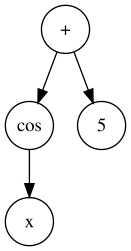
\includegraphics{tree.png}
   \end{center}
      \caption{Indivíduo}
\end{figure}

Foi escolhida essa representação por dois motivos, um por ser exatamente correspondente com as representações utilizadas nos livros-texto. E segundo por ser muito intuitivo a implementação dos métodos que operam sobre os indivíduos.

\subsection{Funções e Terminais}

O conjunto de funções utilizados foi $\{+,-,\cdot, /, \cos, \sin\}$ e os terminais foram
$\{x_i\} \cup \{rand()\}$, onde $0 \le i < n-1$, $n$ é o número de dimensões do problema e $rand()$ é uma função que gera uma constante aleatória entre 2 e 60.

\subsection{Geração da População Inicial}

A população inicial foi gerada pelo método Ramped half-and-half, variando o tamanho dos indivíduos uniformemente de 2 a 7, para aumentar a diversidade inicial.

\subsection{Operadores Genéticos}

Os operadores genéticos utilizados foram o crossover e a mutação, com a opção de ter elitismo ou não. Com elitismo, o melhor entre os filhos e os pais vai para a próxima geração, sem elitismo o melhor filho vai para a próxima geração (Nota-se que isso também é uma forma de elitismo, porém mais amena e como veremos depois, suficiente para tornar a diversidade muito alta). A taxa de crossover é sempre $1-\text{(taxa de mutação)}$.

\subsection{Mecanismo de Seleção}

Para a seleção dos indivíduos foi utilizado o método do torneio, tanto para crossover quanto para mutação.

\subsection{Função de Fitness}

A função de fitness utilizada foi a raiz quadrada do erro quadrático médio normalizada (NRMSE), porém, como será visto na próxima sessão, a convergência estava muito rápida utilizando ela em sua forma padrão. Por isso, para propósitos de seleção, foi utilizada a seguinte função:

\begin{equation}\label{eq:fitness}
fitness(Ind) = \text{NRMSE}(Ind) \cdot \log_\varphi\left(\varphi + \frac{dg}{pi}\right)
\end{equation}

Onde Ind é o indivíduo, $\varphi$ é uma constante, $d$ é quantos indivíduos com o mesmo NRMSE existem na população, $g$ é o número total de gerações, $i$ é o número da geração atual e $p$ é o tamanho da população.

Essa função penaliza fortemente indivíduos com a mesma fitness no começo da execução, mas conforme ela avança o log fica mais próximo de 1. E permite que o algoritmo convirja mais rapidamente. Talvez uma falha nessa fórmula seja que o $log$ não converge de fato para $1$, pois na ultima geração $\frac{dg}{pi} = \frac{d}{p} > 0$, ou seja sempre há uma penalização por falta de diversidade. Por isso foi decidido que a penalização seria removida nas ultimas 5 gerações, para permitir a convergência.

Utilizando essa função de fitness quanto maior $\varphi$ mais rápido o algoritmo converge.

\subsection{Elitismo}

Foi implementado também um mecanismo de elitismo, onde os $k$ melhores indivíduos distintos de uma geração passam para a próxima.

\subsection{Parâmetros}

Os parâmetros ajustáveis pelo usuário são: o tamanho da população, a taxa de mutação, a profundidade minima e máxima, o tamanho do torneio, o número de gerações, $\varphi$ e o número de elites. Todos os parâmetros foram testados na base de dados Synth 1.

\section{Otimização de Parâmetros}

Optou-se por fixar a profundidade minima e máxima como $2$ e $7$ respectivamente, e o número de elites em $5$. Restou então ajustar os outros parâmetros. Para tal para cada variação de parâmetros o algoritmo foi executado $30$ vezes e diversos dados foram coletados. Com esses dados construímos os gráficos que serão apresentados a seguir.


\subsection{Tamanho da População e Número de Gerações}

Aqui testamos todas as combinações entre populações de tamanho $50$, $100$, $200$ e $500$ e número de gerações $50$, $100$, $500$. Foi produzido o gráfico \ref{fig:popgen}. Após uma análise do gráfico em combinação com os tempos de execução \ref{fig:times}, foram escolhidos $500$ para o tamanho da população e $100$ para o número de gerações por apresentar um bom compromisso entre tempo de execução e valor ótimo encontrado.

\begin{figure}[H]
   \begin{center}
   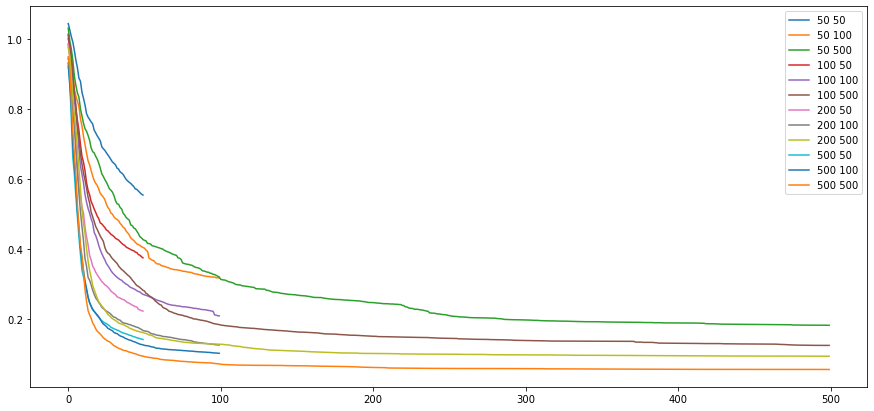
\includegraphics[width=\linewidth]{popgen_best.png}
   \end{center}
      \caption{Melhor indivíduo para diversas combinações de população e geração.}
      \label{fig:popgen}
\end{figure}

\begin{figure}[H]
   \begin{center}
   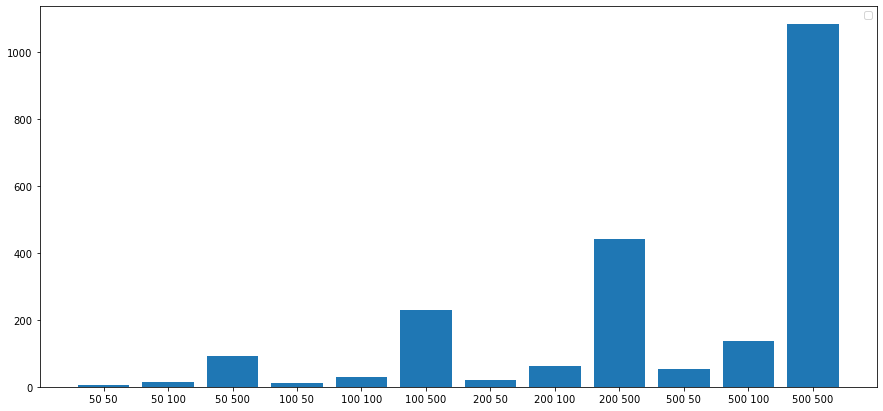
\includegraphics[width=\linewidth]{times.png}
   \end{center}
      \caption{Tempos de execução para diversas combinações de população e geração.}
      \label{fig:times}
\end{figure}

\subsection{Operadores Elitistas}

Agora executamos o algoritmo com e sem operadores elitistas, e produzimos o gráfico \ref{fig:elitism}. Embora o não uso de operadores elitistas tenha produzido indivíduos com melhor fitness, ao olhar a diversidade vimos que os indivíduos não convergem, já com elitismo ocorre uma convergência prematura. Por isso, optamos por utilizar os operadores elitistas, porém com uma função de fitness \ref{eq:fitness} que estimula a diversidade, principalmente no inicio da execução.

\begin{figure}[H]
   \begin{center}
   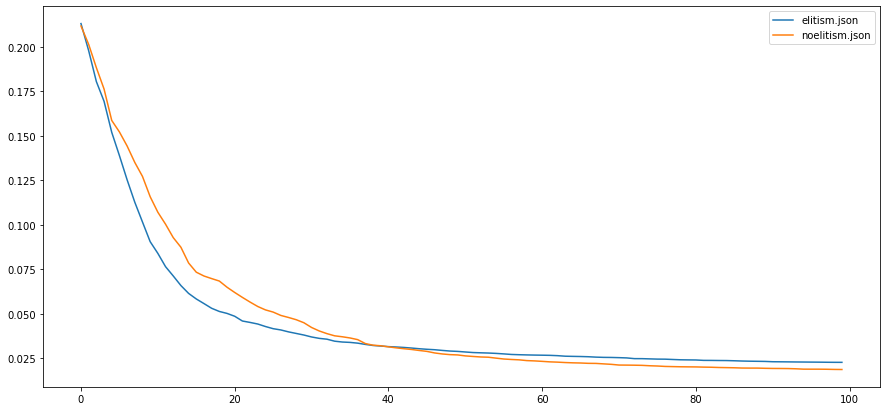
\includegraphics[width=\linewidth]{elitism_best.png}
   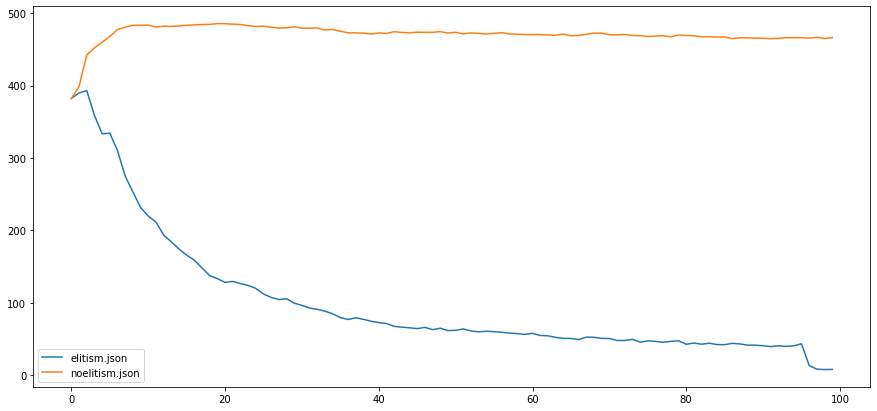
\includegraphics[width=\linewidth]{elitism_div.png}
   \end{center}
      \caption{Melhor indivíduo e diversidade respectivamente quando usando ou não operadores elitistas.}
      \label{fig:elitism}
\end{figure}

\subsection{Taxa de Cruzamento e Mutação}

Como a taxa de cruzamento é $1 - (\text{taxa de mutação})$, para ajustar o cruzamento precisamos apenas ajustar a mutação. Para tal foi produzido o gráfico \ref{fig:mut}. Aqui observamos um fenômeno inesperado, a taxa de mutação não teve grande impacto na diversidade. Para explicar porquê isso acontece foi produzido um outro gráfico \ref{fig:mutbetter} mostrando quantos indivíduos são melhores que os pais, tanto para crossover quanto para mutação.

Nesse gráfico podemos ver que é raro que um indivíduo que passou por uma mutação seja melhor que o indivíduo original, mas ainda sim a diferenciação é suficiente para que se esperasse que maiores taxa de mutação traduzissem em maior diversidade. A explicação proposta para o porquê isso não ocorre é que o cruzamento de subárvores se comporta como uma mutação, então como a redução ou o aumento da taxa de mutação aumenta ou reduz a taxa de cruzamento, essas mudanças se equilibram, gerando resultados similares. Essa hipótese é suportada também pelo gráfico \ref{fig:childbetter}, que mostra quantos filhos passaram para próxima geração por geração. Nele observamos um comportamento similar ao da mutação.

Foi escolhido o valor de $0.1$ para a mutação, arbitrariamente.

\begin{figure}[H]
   \begin{center}
   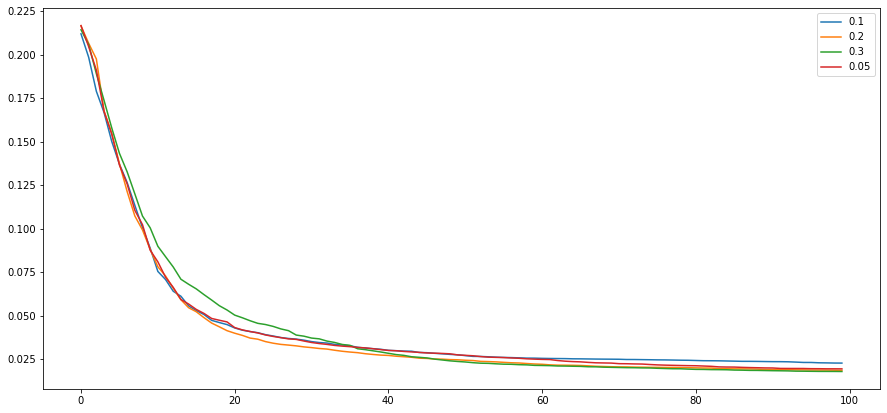
\includegraphics[width=\linewidth]{mut_best.png}
   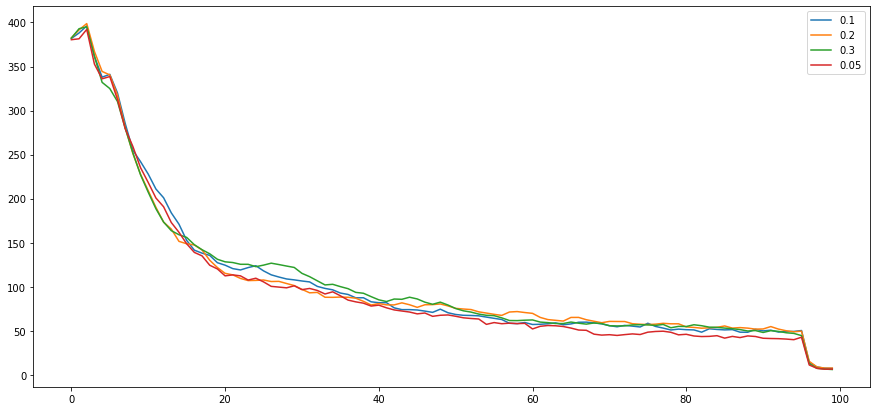
\includegraphics[width=\linewidth]{mut_div.png}
   \end{center}
      \caption{Melhor indivíduo e diversidade respectivamente para diferentes taxas de mutação}
      \label{fig:mut}
\end{figure}

\begin{figure}[H]
   \begin{center}
   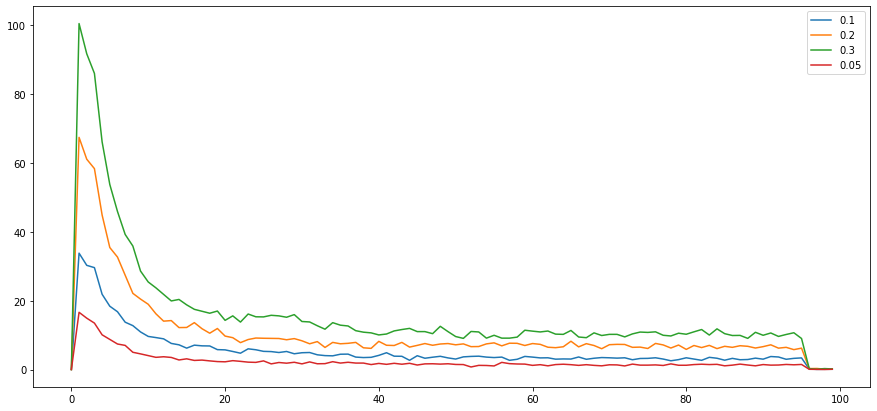
\includegraphics[width=\linewidth]{mut_better.png}
   \end{center}
      \caption{Número de indivíduos cuja mutação foi melhor que o pai por geração.}
      \label{fig:mutbetter}
\end{figure}

\begin{figure}[H]
   \begin{center}
   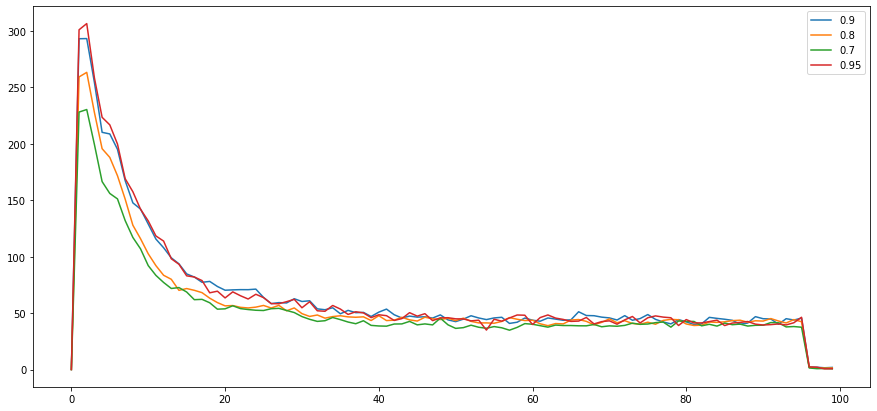
\includegraphics[width=\linewidth]{better_child.png}
   \end{center}
      \caption{Número de filhos gerados por cruzamento que passaram para próxima geração, por geração.}
      \label{fig:childbetter}
\end{figure}

\subsection{$\varphi$}

Em seguida variamos $\varphi$, produzindo o gráfico \ref{fig:phi}. Nele podemos observar que a introdução dessa nova função de fitness realmente promove a diversidade de forma ajustável, e melhora as soluções obtidas. Aqui foi escolhido $\varphi = 1.5$, por apresentar uma curva de diversidade mais suave, e por ter produzido boas soluções ao final de sua execução.

\begin{figure}[h]
   \begin{center}
   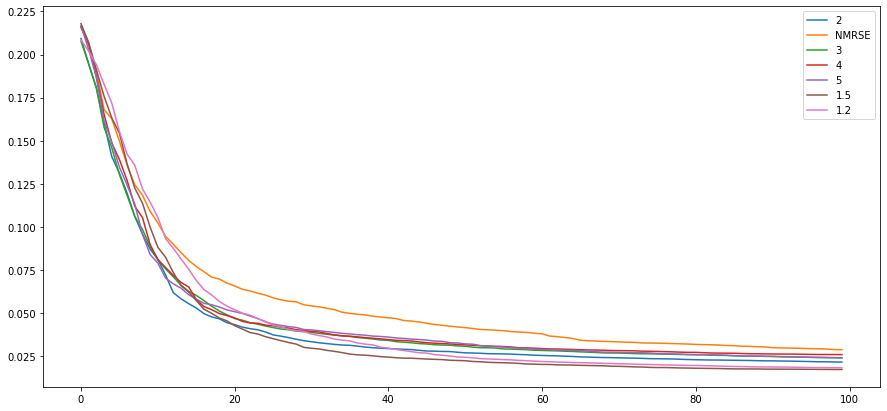
\includegraphics[width=\linewidth]{phi_best.png}
   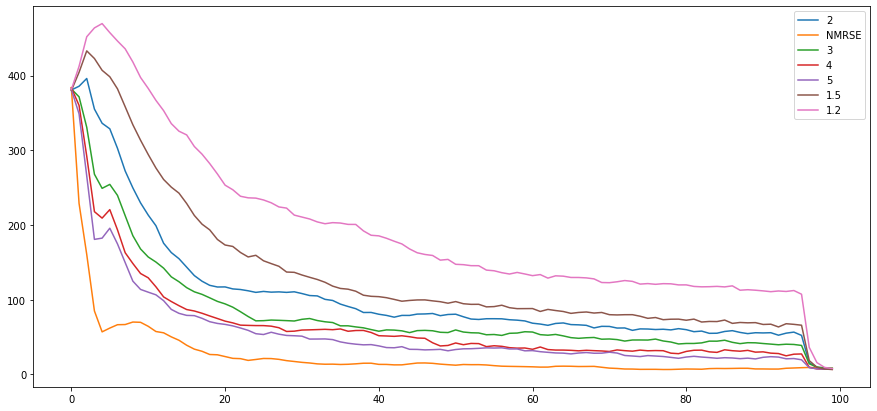
\includegraphics[width=\linewidth]{phi_div.png}
   \end{center}
      \caption{Melhor indivíduo e diversidade respectivamente para diferentes valores de $\varphi$}
      \label{fig:phi}
\end{figure}



\subsection{Tamanho do Torneio}

Nessa etapa o algoritmo foi executado para diferentes tamanhos de torneio e o gráfico \ref{fig:tourn} foi produzido. Note que, mais uma vez, algo inesperado ocorreu, tamanhos menores de torneio convergiram mais rapidamente, que é exatamente o oposto do que seria esperado. Esse efeito se torna mais aparente quanto mais avançadas as gerações.

Talvez o motivo seja que torneios maiores aumentem a chance que indivíduos repetidos sejam escolhidos para a próxima geração, mas isso faz com que esses indivíduos sejam mais penalizados pela função de fitness \ref{eq:fitness}, fazendo com que eles não sejam escolhidos para a próxima geração, promovendo uma maior diversidade. Mas isso não explica porquê para torneios de tamanho $2$ a convergência seja tão mais rápida.

Para o objetivo de selecionar o melhor parâmetro, torneios de tamanho $2$ performaram bem quanto ao fitness, e apresentaram uma curva de diversidade próxima do que estava sendo procurado, portanto foi escolhido esse valor.


\begin{figure}[H]
   \begin{center}
   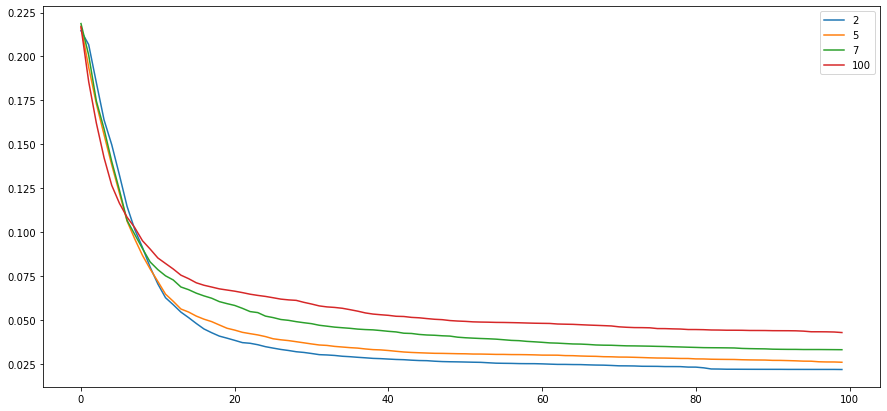
\includegraphics[width=\linewidth]{tourn_best.png}
   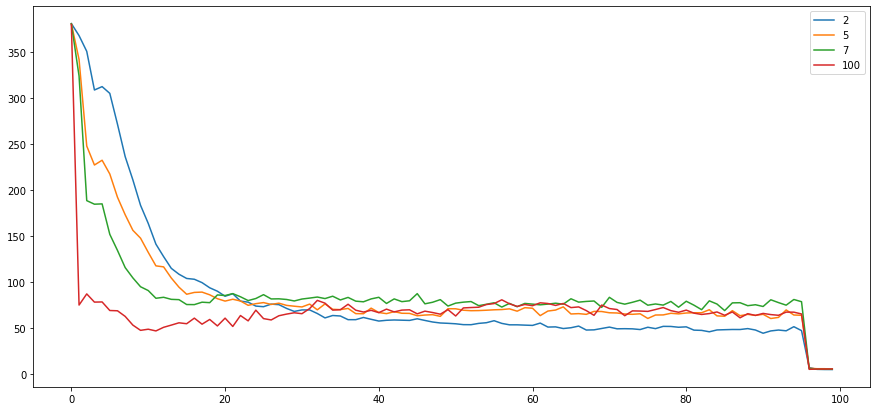
\includegraphics[width=\linewidth]{tourn_div.png}
   \end{center}
      \caption{Melhor indivíduo e diversidade respectivamente para diferentes tamanhos de torneio}
      \label{fig:tourn}
\end{figure}

\subsection{Parâmetros Finais}

A tabela \ref{tab:param} apresenta os parâmetros escolhidos. E o gráfico \ref{fig:final} apresenta o resultado da execução com esses parâmetros.

\begin{table}[H]
   \caption{Parâmetros finais}
   \centering
   \begin{tabular}{|c|c|}
    \hline
    Parâmetro & Valor \\
    \hline\hline
    Tamanho da População & $500$ \\
    \hline
    Número de Gerações & $100$ \\
    \hline
    Operadores Elitistas & Sim \\
    \hline
    $\varphi$ & $1.5$ \\
    \hline
    Taxa de Cruzamento & $0.9$ \\
    \hline
    Taxa de Mutação & $0.1$ \\
    \hline
    Tamanho do Torneio & $2$ \\
    \hline

   \end{tabular}
   \label{tab:param}

\end{table}

\begin{figure}[H]
   \begin{center}
   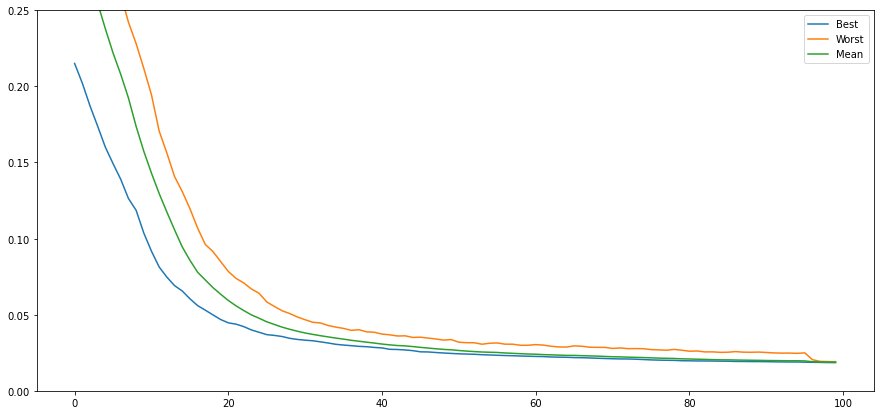
\includegraphics[width=\linewidth]{final.png}
   \end{center}
      \caption{Média do melhor, pior, e média dos indivíduos em 30 execuções do algoritmo com os parâmetros descritos na tabela \ref{tab:param}}
      \label{fig:final}
\end{figure}

Na sessão seguinte iremos descrever os resultados do algoritmo para os três conjuntos de dados.

\section{Resultados}

A seguir apresentamos estatísticas descritivas das regressões para as bases de dados Synth $1$, Synth $2$ e Concrete, executadas $30$ vezes cada uma. Além disso foram produzidos os gráficos \ref{fig:surfaces} da melhor solução para Synth $1$ e Synth $2$.

A tabela \ref{tab:train} mostra as estatísticas descritivas das soluções encontradas medindo a fitness sobre o conjunto de treinamento. E a tabela \ref{tab:test} mostra as mesmas estatísticas para o conjunto de teste. Aqui mais uma vez como tem sido o tema desse trabalho, ocorre algo inesperado: Em média as soluções para o conjunto de dados Concrete performaram bem melhor sob o conjunto de teste do que sob o conjunto de treinamento, e esse comportamento foi o mesmo em várias execuções.

Uma explicação possível é que os pontos do conjunto de teste se encontram em regiões similares, para as quais as soluções produzidas pela programação genética se aproximam bem.

\begin{table}[h]
   \caption{Estatísticas descritivas sobre os conjuntos de treinamento de cada conjunto de dados}
\centering
\begin{tabular}{|l|r|r|r|}
   \hline
   & Mean & std & min \\
   \hline
   Synth 1 & 0.014906 & 0.009255 & 0.000000 \\
   Synth 2 & 0.204465 & 0.031793 & 0.120785 \\
   Concrete & 1.166887 & 0.132183 & 0.914956 \\
  \hline
\end{tabular}

\begin{tabular}{|l|r|r|r|}
   \hline
   & 50\% & 75\% & 95\% \\
   \hline
   Synth 1 & 0.014360 & 0.022611 & 0.027911 \\
   Synth 2 & 0.198443 & 0.226986 & 0.253099 \\
   Concrete & 1.167574 & 1.258472 & 1.404362 \\
  \hline
\end{tabular}
\label{tab:train}
\end{table}


\begin{table}[h]
   \caption{Estatísticas descritivas sobre os conjuntos de teste de cada conjunto de dados}
\centering
\begin{tabular}{|l|r|r|r|}
   \hline
   & Mean & std & min \\
   \hline
   Synth 1 & 0.115204 & 0.205079 & 0.000000 \\
   Synth 2 & 1.231052 & 2.226418 & 0.246288 \\
   Concrete & 0.581462 & 0.070561 & 0.447135 \\
  \hline
\end{tabular}

\begin{tabular}{|l|r|r|r|}
   \hline
   & 50\% & 75\% & 95\% \\
   \hline
   Synth 1 & 0.059018 & 0.142452 & 0.188007 \\
   Synth 2 & 0.563888 & 0.623724 & 6.313074 \\
   Concrete & 0.576918 & 0.620111 & 0.702474 \\
  \hline
\end{tabular}
\label{tab:test}
\end{table}


\begin{figure}[H]
   \begin{tabular}{cc}
   Ground Truth & Our Solution \\
   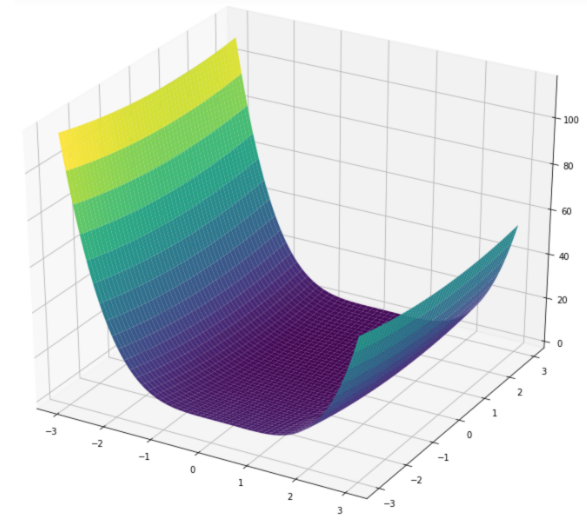
\includegraphics[width=.5\linewidth]{synth1_ground.png} & 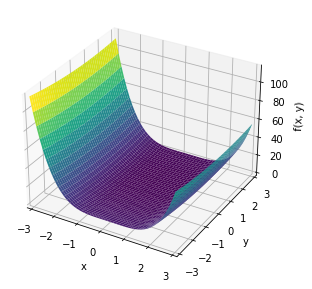
\includegraphics[width=.5\linewidth]{synth1_plot.png}\\

   Synth1  \\
   \hline
   Synth2  \\
   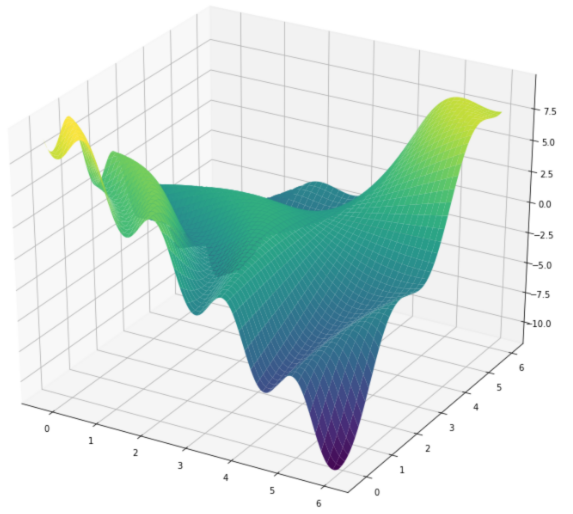
\includegraphics[width=.5\linewidth]{synth2_ground.png} & 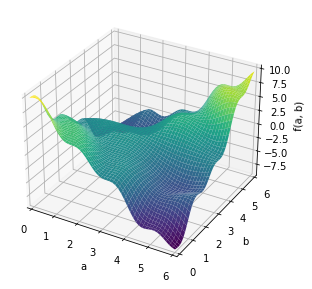
\includegraphics[width=.5\linewidth]{synth2_plot.png}
   \end{tabular}
      \caption{Gráficos da melhor solução encontrada para Synth 1 (Acima) e Synth 2 (Abaixo)}
      \label{fig:surfaces}
\end{figure}


\section{Conclusão}

O algoritmo proposto com os parâmetros levantados apresentou bons resultados em geral no percentil $.75$ para os conjuntos de teste. Porém no percentil $.95$ para o conjunto de dados Synth 2 os resultados foram bem piores. Isso pode indicar um problema de suficiência e parcimônia, talvez seja o caso que não foram providas todas as funções necessárias para representar a solução, ou que há funções de mais. Porém olhando para a mediana (Percentil $.5$) que apresentou um resultado satisfatório, parece que o problema talvez seja de exploração do espaço de soluções.


Portanto futuramente seria adequado testar outras medidas para estimular a diversidade, talvez com um fitness sharing mais abrangente, penalizando soluções na mesma região de busca. Também faria sentido testar outros conjuntos de funções, por exemplo, talvez não seja necessário ter ambos seno e cosseno no conjunto desde que se inclua algumas frações de $\pi$ como terminais, pois $\sin(x+\frac{\pi}{2}) = \cos(x)$.







\end{document}
